\documentclass[../root]{subfiles}
\graphicspath{{_images/}{../_images/}}

\begin{document}

    \chapter{Cognitive Mobility: Labor Market Responses to Supply Shocks in the Space of Ideas}

    \begin{shortsummary}
        \begin{itemize}
            \item \authoryear{Borjas2015} 
            \item \RQ{How supply shock of Soviet-mathematicians impact on the cognitive mobility of  American-mathematicians?}
            \item \answer{The authors use panel data of American-mathematicians' paper to estimate the impact of supply shock.}
            \item \result{Supply shock lead to harder competitive. American mathematicians avoid to choose Soviet-style topics.}
        \end{itemize}
    \end{shortsummary}

    \section{Introduction}
   The labor mobility  have been studied  many times and it is motivated to explain the impact on labor market.    
   
   This paper treat cognitive mobility. Labor mobility lead to move idea space. 
   
   For example, Borjas and Doran (2012) exposure supply shock of mathematician in United States after collapse Soviet Union led to decrease of output.
   
   The authors examine the impact of supply shock on American mathematicians.
   
   Standard model suggest the supply  response can be either positive or negative impact on cognitive , depending on whether spillover effect. 
   
   {\bf Research question and how to answer it}
   \begin{itemize}
       \item Does cognitive mobility cause spillover after supply shock?
       \item The data consist of all publications by American mathematicians between 1940 and 2009, including detailed information on the "field" of each publication.
   \end{itemize}
   
   
   The authors find the supply shock generate cognitive mobility response.
   \begin{itemize}
       \item They reveal to mathematician who move to different filed  take longer to produce their next paper than who don't move.
       \item Soviet inflow lead to harder competition.
       \item The cost of moving to another field are correlated with cognitive mobility and Soviet inflow increased those for a significant number of American mathematicians.  
       \item Experienced mathematicians were relatively less likely to choose Soviet field than were younger or less productive mathematicians. 
   \end{itemize}
   
   These results means the net benefit from human capital spillovers were higher.
   
    \section{Conceptual Framework}
    
    The basic model of knowledge production is inspire by the model that human capital externalities affect the productivity of specific workers.
    
    The production function for "mathematical production" in United States, $Y$, depends on the idea $I$, the stock of capital $K$ used as input, and the stock of mathematicians $L$. 
    
    \begin{align}
        Y=I^{\phi} (K^{\alpha}L^{1-\alpha}),
    \end{align}
    where $\phi$ gives the "externalities elasticity".
    
    We assume that the stock of idea is proportion to the size of workforce.
    The short  and long-run effect on a supply shock ($m=d \ \mbox{log}$ \ L) on the marginal product of mathematicians are 
    
    \begin{align}
        d \ \mbox{log} \ MP_L = 
            \begin{cases}
                (\phi - \alpha)m & \mbox{if}\ d\ \mbox{log} \ K=0 \\
                \phi m & \mbox{if }\ d\ \mbox{log} \ K =m
            \end{cases}
    \end{align}
    
    \begin{itemize}
        \item  The sign of Short-run effect dependent on the size of spillover and traditional competitive.
        \item The long-run effect will be positive, if spillover effect exist.
    \end{itemize}
   
   Next, we consider cognitive mobility. Mathematicians is not homogeneous and composed by distinct "field".
   
   Suppose that there are F distinct mathematical fields, and $L$ are expressed as follow
   \begin{align}
       L = (I^{\theta}_1 L^{\beta}_1+ \cdot \cdot + I^{\theta}_L L^{\beta}_L)^{\frac{1}{\beta}},
   \end{align}
    where elasticity of substitution between mathematicians in different field is $\sigma = \frac{1}{1-\beta}$ .
    
    Let $m_S$ and $m_A$ give the percentage change in the number of  Soviet-style and American-style mathematicians and because of Soviet inflow $m_S > m_A$. 
    
    The impact of labor supply shock on the relative productivity  in these two area is given by
    
    \begin{align}
        d \ \mbox{log }\ MP_S - d \ \mbox{log }\ MP_A = (\theta-\frac{1}{\sigma})(m_S - m_A) 
    \end{align}
    
    in both the short and long run.
    
    The net impact of the sign of supply shock depend on the size of local externaity elasticity  $\theta$ and  competitive effect measured by the inverse of the elasticity of substitution. 
    
    \begin{itemize}
        \item Let $MP_{iA}$ and $MP_{iS}$ denote the marginal product of mathematicians in the Soviet- and American- style field, respectively.
        \item Before the collapse of the Soviet Union, income-maximizing mathematicians decide to conduct in Soviet-dominated field if $MP_{iS}>MP_{iA}$. 
    \end{itemize}
    
    Let $\gamma_i$ the net supply shock on productivity mathematicians $i$.
    After the supply shock, a Soviet-style mathematicians will engage cognitive mobility and conduct American-style research only if
    \begin{align}
        MP_{iS} + \gamma_i < MP_{iA}- C_i,
    \end{align} 
    where $C_i$ gives the cost of cognitive mobility. We assume that these costs of cognitive mobility is strictly positive.
    
    The preshock reveals preference mathematicians $i$ implies they switch to American -style research iff 
    \begin{align}
        \gamma_i < -C_i
    \end{align}
    
    Since mobility cost is positive, they move only if $gamma_i$ is strictly negative.
    
    Similary, consider the cognitive mobility decision of mathematicians who are conducting American-style research prior to the supply shock. 
    \begin{itemize}
        \item The mathematicians must satisfy $MP_{iA} > MP_{iS}$
        \item Mathematicians in this group will switch to Soviet-style research after the supply shock if (7) condition is satisfied.
        \item If these mathematicians move to Soviet-style research, follow (8) condition is satisfied. 
    \end{itemize}
    
    \begin{align}
         MP_{iS} + \gamma_i -C_i > MP_{iA}
     \end{align}
     
     \begin{align}
         \gamma_i > C_i
     \end{align}
     
     \begin{itemize}
         \item Cognitive mobility will be observed only if the net spillover numerically large regardless of sign.
     \end{itemize}
     
     \section{Historical Context and Data}
     They use the data as the research decision made by mathematicians in the United State prior and after collapse of Soviet Union.
     
     Borjas and Doran(2012) document after a long period of infrequent contract between Soviet and Western mathematicians, over 1000 Soviet mathematicians (or roughly 10 \% of the stock) left the Soviet Union after 1992. 
     
     This particular event has a number of key feature in their identification strategy:
     
     \begin{enumerate}
         \item Exogenous migration Soviet to America occur in 1900-1901.
         \item The supply shock was large.
         \item The contract between Soviet and Western mathematicians was infrequently during the decades of Soviet communities rules.
         \item The impact of supply shocks was differently each field.  
     \end{enumerate}
     
     The authors' empirical strategy is to compute the degree of cognitive mobility experienced by these two group of American mathematicians both before and after the shock.
     
    They use the American Mathematical Society's MathSciNet archives as the publish data.
    
    AMS provide follow data.
    \begin{itemize}
        \item The number of the papers published by every mathematicians in the world, by field and year, since 1939.
        \item The mathematicians 's institution  affiliation at the time the paper published. 
    \end{itemize}
    
     The authors define the person as "American"  if more than half of these publications used an American affiliation. 
     
     They construct a panel in which an observation represent a mathematician/paper permutation.
     Their data describe the entire publication history of American mathematicians between 1940 and 2009. 
     
     There are 525,944.
     
     Table 1 represents the number and the percentage of mathematicians Pre-1992 and Post-1992.
    \begin{figure}
        \centering
        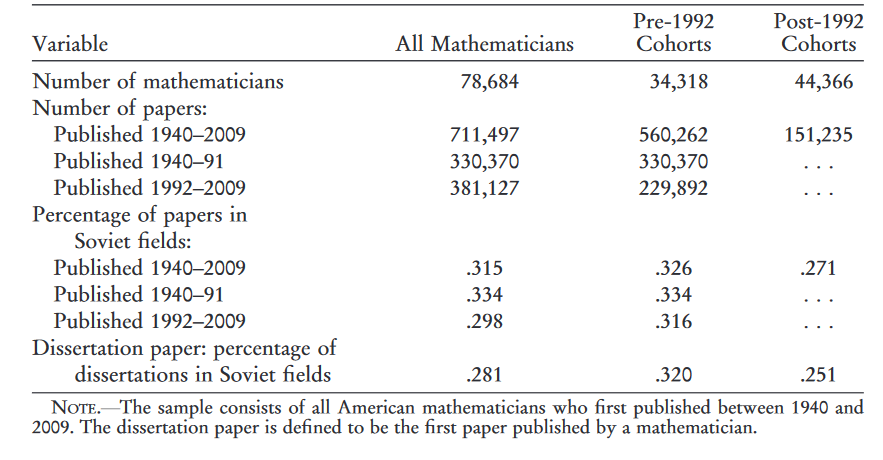
\includegraphics[width = \linewidth]{_images/0918sugiyama/Table_1.png}
        \caption{Summary Statistics, Sample of American Mathematicians}
        \label{fig:my_label}
    \end{figure}
    
    They examine the trends in the field distribution of papers publication  by American mathematicians.
    
    Table2 represents "Soviet-field" and the percentage of "Soviet-field"papers. 
    \begin{figure}
        \centering
        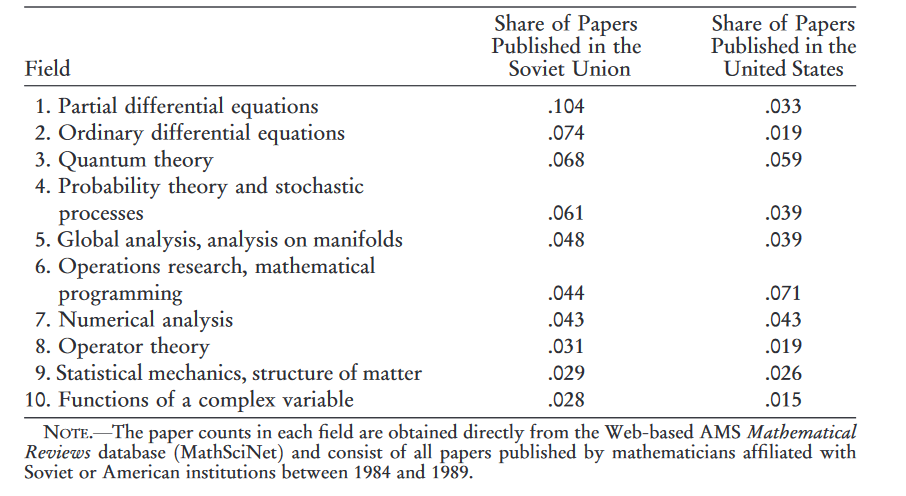
\includegraphics[width = \linewidth]{_images/0918sugiyama/Table_2.png}
        \caption{Main Fields of Publication in the Soviet Union, 1984-89}
        \label{fig:my_label}
    \end{figure}
   
   
   \section{The Determinants of Cognitive Mobility}
   
   \begin{itemize}
       \item "preparation spell" means the timing while  between a mathematicians complete the paper and subsequent paper is submitted.
       \item During preparation spell, mathematicians decide to move or stay the location (field).
       \item Supply shock lead some mathematicians change their filed.
   \end{itemize}
     
     Supply shock could increase the productivity for mathematicians already resident in that field and may increase the cost to move to that field.
   
   This section examine follow two things
   \begin{enumerate}
       \item  Which factor induce a mathematicians to move to different field in response to supply shock.
       \item Does cognitive mobility represent movement toward the research question favored by newcomers or away from them? 
   \end{enumerate}
       
   Section II show supply shock cause the human capital spillover and the increased competitive.
   The direction of cognitive mobility flow provide information about which of these two effect is dominant.
   
   {\bf Examine the locational choices in in idea space}
   \begin{itemize}
        \item Sample is American mathematicians who entered active research activity prior 1992.
        \item They define two distinct group: Those who pre-1992 paper was on a Soviet-style topic and those who pre-1992 paper was not.
        \item They identify 73 mathematical fields as (i) 10 Soviet-style fields that were the most populated in the Soviet Union prior to the collapse; and (ii) 63 American-style fields.
    \end{itemize}
   
   They don't interpret The move to consecutive field is not cognitive mobility.
   
   They use pre-supply shock data to examine the probability of the cognitive mobility of American mathematicians and check whether the probability of after supply shock  is same or not.
   
   Panel A of figure 1 show the cognitive mobility trends, the probability that a paper written in year $t$ is in a different field than the dissertation.  
   \begin{figure}
        \centering
        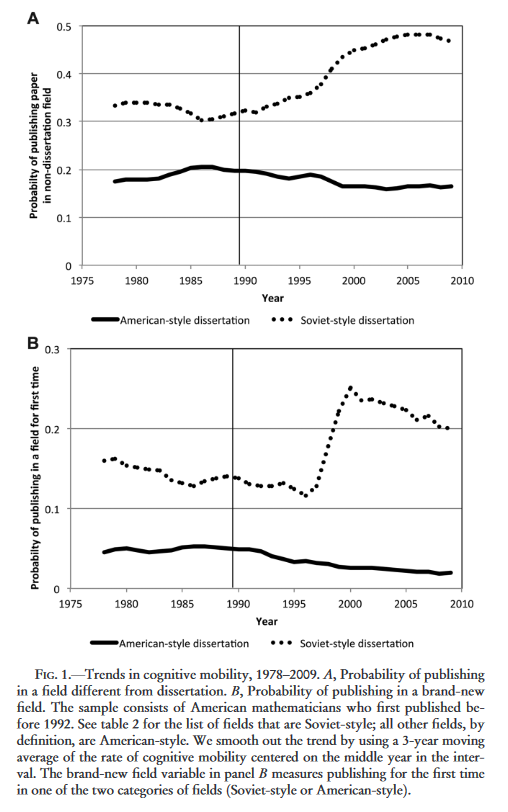
\includegraphics[width = \linewidth]{_images/0918sugiyama/Figure_1.png}
        \caption{Trend in mobility}
        \label{fig:my_label}
    \end{figure}
    
    \begin{itemize}
        \item Panel A show the probability that mathematicians who wrote Soviet-style paper did cognitive mobility increased. 
        \item The result of panel A suggest the net spillover effect must be strongly negative overweight the cognitive costs. 
    \end{itemize}
    
    Panel B of figure 1 using a measure that indicate whether a mathematicians entered a field which he had never publish before.
    
    \begin{itemize}
        \item Clearly shown, there was a sharply increase in the tendency of Soviet-style mathematicians to explore to other research area for the first time.
        \item The timing gap between Soviet collapse and the start increasing means the duration that the mathematicians retool mathematical skills for another fields.
    \end{itemize}
    To conduct the estimation the effect of various background characteristics, they estimate the linear probability regression model 
    \begin{align}
        p_{in}(t) = \delta_i + \delta_t + \theta (T_i \times S_i) +Z_i \beta +\epsilon,
    \end{align}
    
    where $p_{in}$ is the probability of cognitive mobility from the dissertation to paper $n$ published by mathematicians $i$ in calendar year $t$; $T_i$ is a dummy variable indicating if the paper was published after 1992; $S_i$ is a dummy variable indicating if the mathematician's dissertation is Soviet-style field.  
    
    $Z_i$ is mathematicians' characteristics factor:
    \begin{itemize}
        \item In column 1, they control the year of mathematicians' experience.
        \item In column 2, they add some variables: an indicator of of whether the mathematicians was likely to be tenured as of 1992 and the mathematicians' ratio of ratio.
        \item In column 2, they add individual ability.
    \end{itemize}
    
    \begin{figure}
        \centering
        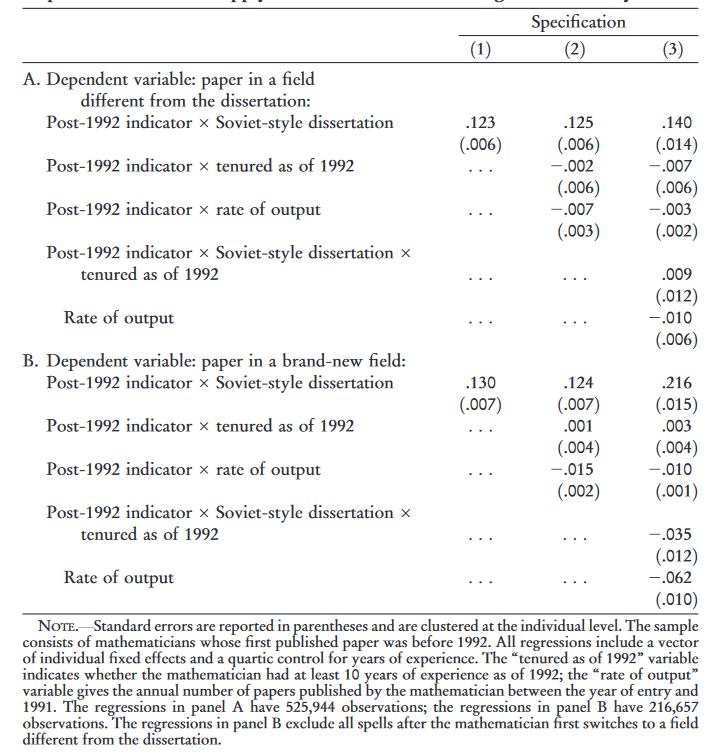
\includegraphics[width = \linewidth]{_images/0918sugiyama/Table_3.png}
        \caption{Table 3. Impact of the Soviet Supply Shock on the Rate of Cognitive Mobility}
        \label{fig:my_label}
    \end{figure}
    
    Regardless the specification, the supply shock lead to a substantial increase in cognitive mobility from Soviet-style field into American-style field.
    
    From the results, the probability cognitive mobility rose remarkedly for the "average" Soviet-style but did not change for high-ability Soviet-mathematicians.
    
    Table 4 represent the robustness results of in table 3.
    \begin{figure}
        \centering
        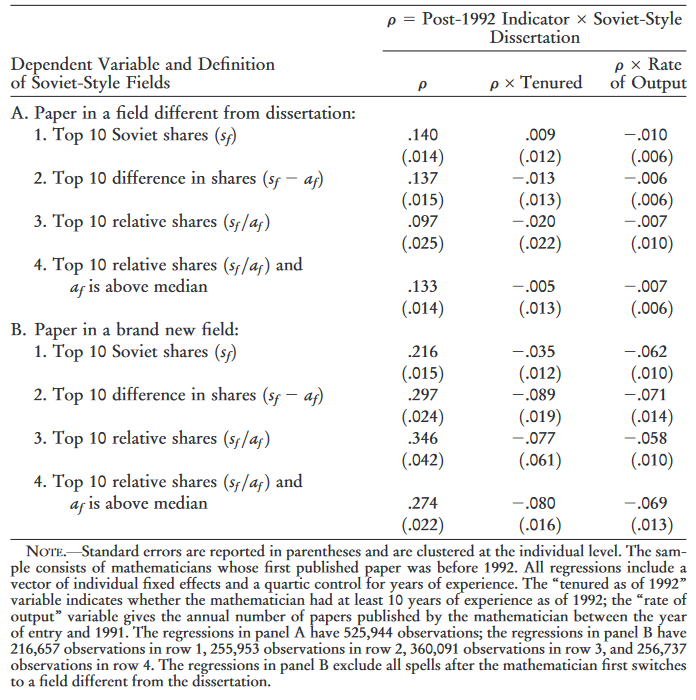
\includegraphics[width = \linewidth]{_images/0918sugiyama/Table_4.png}
        \caption{Table 4. Sensitivity of Results to Alternative Definitions of Soviet-Style Fields}
        \label{fig:my_label}
    \end{figure}
    
    $s_f$ and $a_f $ means the share of pre-1989 papers published in field $f$ in Soviet Union and United States. 
    \begin{itemize}
        \item Row 2 use the definition as $s_f - a_f$. 
        \item Row 3 use the definition as $s_f/a_f$.
        \item Eow 4 use the definition as $s_f/a_f$ and in particular $a_f$ is above the median.
    \end{itemize}
    
    The results in row 1-4 is similar.
    
    They construct measure of cognitive distance and estimate using this index.
    
    The index of similarity for mathematicians $i$ is defined by 
    \begin{align}
        D_i = 1- \frac{1}{2}\sum_f |a_{if} - s_f|,
    \end{align}
    where $a_if$ is the share of the paper that American mathematicians $i$ published in the filed $f$ and $s_f$ is the share of all Soviet paper published in $f$ before the collapse of the Soviet Union. 
    
    The paper of similarity of every paper $n$ is 
    \begin{align}
        D_{ifn} (t) = s_f
    \end{align}
    
    From above notation, they compute the distance between $n$ the paper and the dissertation: $\Delata_{in}(t) = D_{ifn}(t - D_{if1}(t'))$.  
    Panel A of figure 2 illustrate the trends in the absolute value of cognitive distance.
    
    \begin{figure}
        \centering
        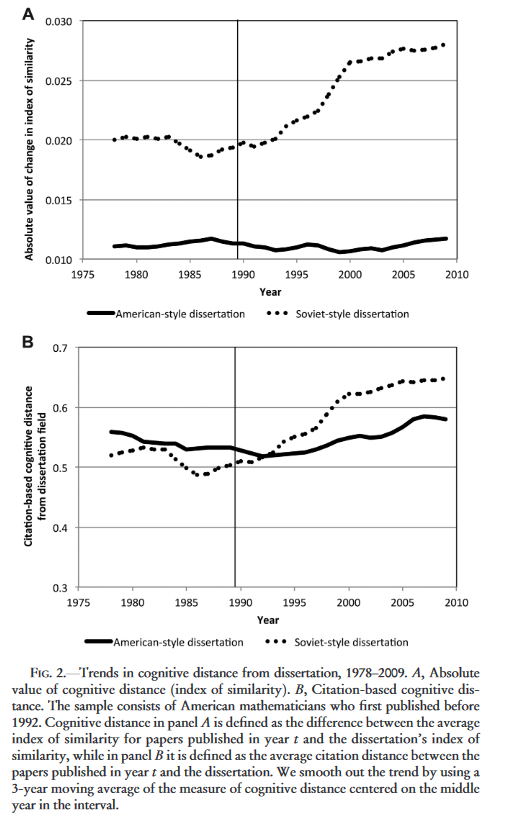
\includegraphics[width = \linewidth]{_images/0918sugiyama/Figure_2.png}
        \caption{Figure_2 Trends in cognitive distance from dissertation,}
        \label{fig:my_label}
    \end{figure}
    
    The basic regression specification yields 
    \begin{align}
        |\Delta_{in}(t)| = \delta_i + \delta_t +\underset{(.008)}{.097} (T_i \times D_{if1}) \\
        \Delta_{in}(t) = \delta_i + \delta_t -\underset{(.008)}{.098} (T_i \times D_{if1})
    \end{align}
    
    \begin{itemize}
        \item Equation (12) shows if the mathematicians wrote more Soviet-style dissertation, the distance between the nth paper and the dissertation is increase after 1992.
        \item Equation (13) shows the Soviet-style mathematicians move to more far way fields.
    \end{itemize}
    
    Next measure of cognitive distance is frequency with witch field cites.
    
    \begin{align}
        \Omega_{fg}=\frac{c_{ff}-c_{fg}} {max(c_{ff}-c_{fg})} ,
    \end{align}
    where $c_{fg}$ is the share of citations made by papers published in field $f$ to paper published in field $g$.
    
    The index $\Omega_{fg}$ equal zero when the mathematicians "travels" from one paper in field $f$ to $g$.
    
    The data show .99\% citation is between same field an donly the  "closest"  2 \% of "field pair".
    
    Let $\Omega_{in}(t)$ denote the distance between n th paper and dissertation paper. 
    
    Panel B of figure 2 illustrates of this measure cognitive distance.
    
    The basic regression specification yields
    \begin{align}
        \Omega_{in}(t) = \delta_i + \delta_t + \underset{(.006)}{.043}(T_i \times S_i)
    \end{align}
    
    Equation (15) show the Soviet-style mathematicians moved to other fields after 1992.
    
    The important check is that the above results are really induced by immigrants-supply shock. 
    They estimate whether American mathematicians have higher rate of cognitive mobility from the Soviet-style filed than other countries' mathematicians or not.   
    
    \begin{align}
        p_{in} (t) = \delta_i + \delta_t + \theta(T_i \times S_i) + \theta(T_i \times S_i \times USA_i) + Z_i \beta +\epsilon
    \end{align}
    
    Table 5 represent the results of this estimation.
    
    \begin{figure}
        \centering
        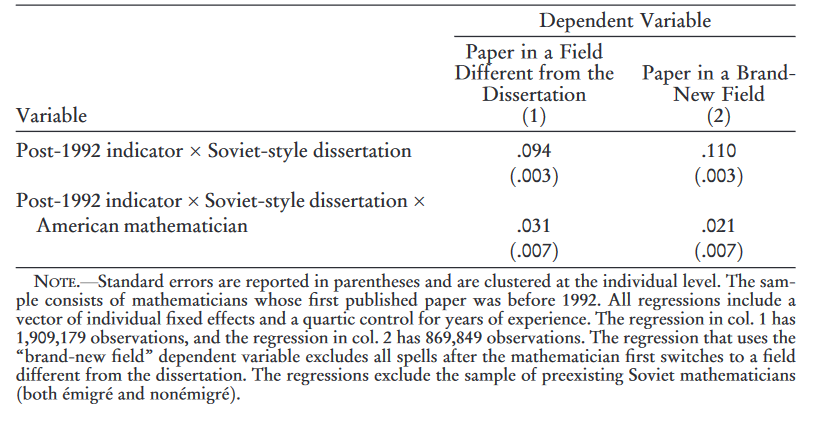
\includegraphics[width = \linewidth]{_images/0918sugiyama/Table_5.png}
        \caption{Table 5. Relative Impact of the Soviet Supply Shock on American Mathematicians}
        \label{fig:my_label}
    \end{figure}
    
    American mathematicians had higher rate of cognitive mobility from the Soviet-style filed than other countries' mathematicians.
    
    \section{The Costs of Cognitive Mobility}
    Cognitive mobility may be costly and the time should need longer time to publish next paper. 
    
    The supply shock potentially increase the cognitive costs in two distinct ways.
    \begin{enumerate}
        \item It increase the propensity for cognitive mobility among American-style mathematicians.
        \item The clustering of large number of Soviet mathematicians in specific locations in idea space could increase the length of the preparation spell for cognitive movers.
    \end{enumerate}
    Table 6 summaries the length of preparation spell for American- and Soviet- style mathematicians.
    
    They define the duration of preparation spells as the length of time elapsed  between any two consecutive papers. 
    
    \begin{itemize}
        \item Panel A show the preparation spell before and after collapse.
        \item Panel B show supply shock increase the duration of preparation spells.
    \end{itemize}
    
    \begin{figure}
        \centering
        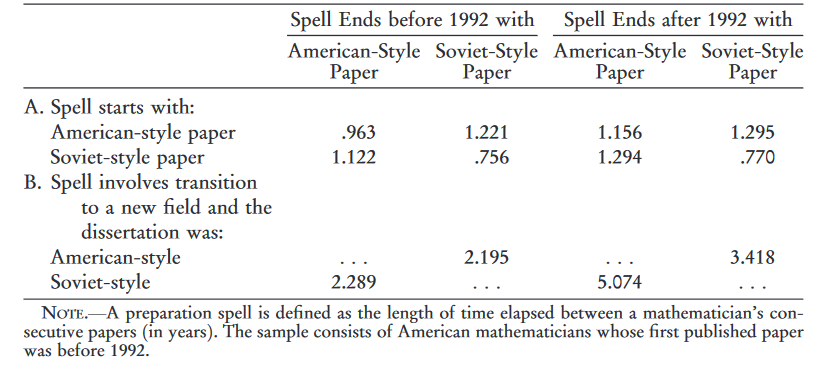
\includegraphics[width = \linewidth]{_images/0918sugiyama/Table_6.png}
        \caption{Table 6. Summary Statistics of the Duration of Preparation Spells}
        \label{fig:my_label}
    \end{figure}
    
    They examine the sensitivity of of these finding controlling for various characteristics by estimating the regression model
    \begin{align}
        y_{in} (t) = &\delta_i + \delta_t + \theta_0(S_i \times F_{in}) + \theta_1 (T_i \times S_i) + \theta_2 (T_i \times S_i \times F_{in})  \nonumber \\ 
        &+ \kappa_0 (A_i \times F_{in}) + \kappa(T_i \times A_i) +\kappa_2 (T_i \times A_i \times F_{in}) + Z_i \beta + \epsilon,
    \end{align}
    
    where $y_{in}(t)$  is the duration of the preparation spells that cumulative in mathematicians $i$ publishing paper $n$ at timing $t$.
    \begin{itemize}
        \item $F_{in}$  is dummy variable indicating if the paper is the field that the mathematicians had not previously explored.
        \item $A_i = 1- S_i$.
    \end{itemize}
    
    Table 7 represent the results of this regression.
    \begin{figure}
        \centering
        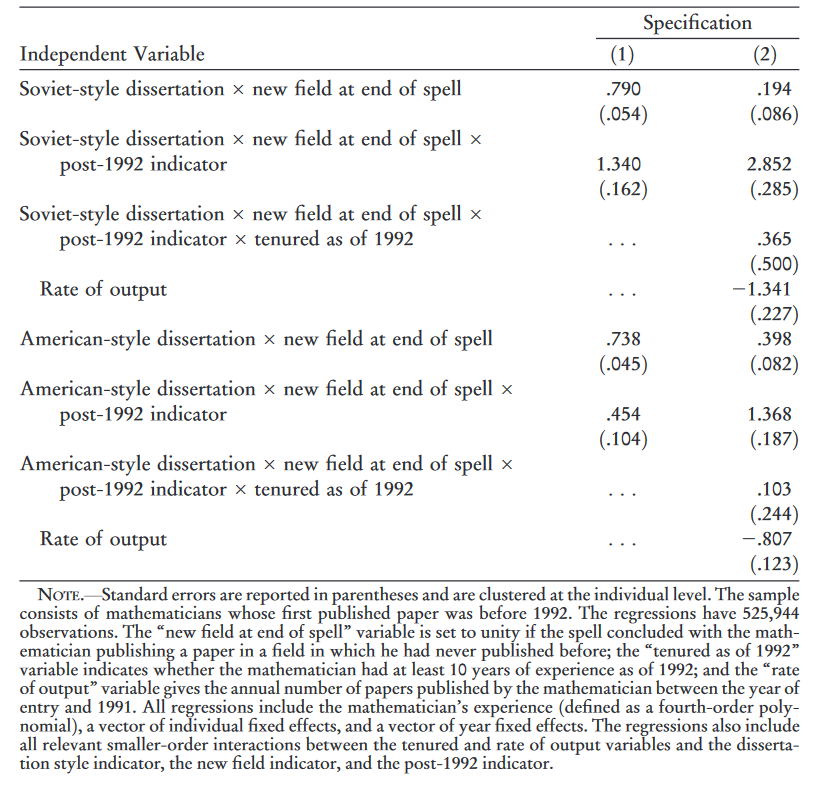
\includegraphics[width = \linewidth]{_images/0918sugiyama/Table_7.png}
        \caption{Table 7. Impact of the Soviet Supply Shock on the Duration of Preparation Spells}
        \label{fig:my_label}
    \end{figure}
    
    \begin{itemize}
        \item First column show the results controlling only the years of experience, and Soviet-style mathematicians use more time to switch new field than American-style mathematicians.
        \item Column 2 show the add the variable of tenured as indicator of ability. The results show that supply shock increase the duration of preparation spells of low ability mathematicians. 
    \end{itemize}
    
    The above increase is consist with two causal scenario:
    \begin{enumerate}
        \item The supply shock made it relatively more difficult for Soviet-style mathematicians to produce output and some of them seek a new location.
        \item The supply shock lead the Soviet-style mathematicians to move brand new field and it need longer time to produce first paper in new field. 
    \end{enumerate}
    Under the first scenario, time lags cause cognitive mobility. And under second scenario, the causation is reverse. 
    
    But, in their data, they cannot distinguish the causality between cognitive mobility and time lags.
    
    The reason why the high ability mathematicians didn't have tendency choosing cognitive mobility may be explained follow two ways:
    \begin{itemize}
        \item The high ability mathematicians benefited from the spillover caused by supply shock.
        \item The high ability mathematicians had the highest cognitive mobility.
    \end{itemize}
    
    The results which is shown in this chapter strongly suggest the high ability mathematicians had lower cognitive mobility.
    
    \section{Field Choice of New Cohorts}
    The authors have examined the impact of supply shock on "preexisting" mathematicians. In this section, they estimate the impact on new comers.
    
    \begin{itemize}
        \item They examine the the field choice of the first published by each mathematicians to show the "cohorts effect".
        \item They control the group of mathematicians "rest of the world".
    \end{itemize}
    
    Figure 3 show the number of Soviet-style dissertation were decreasing in after 1990 cohort. 
    \begin{figure}
        \centering
        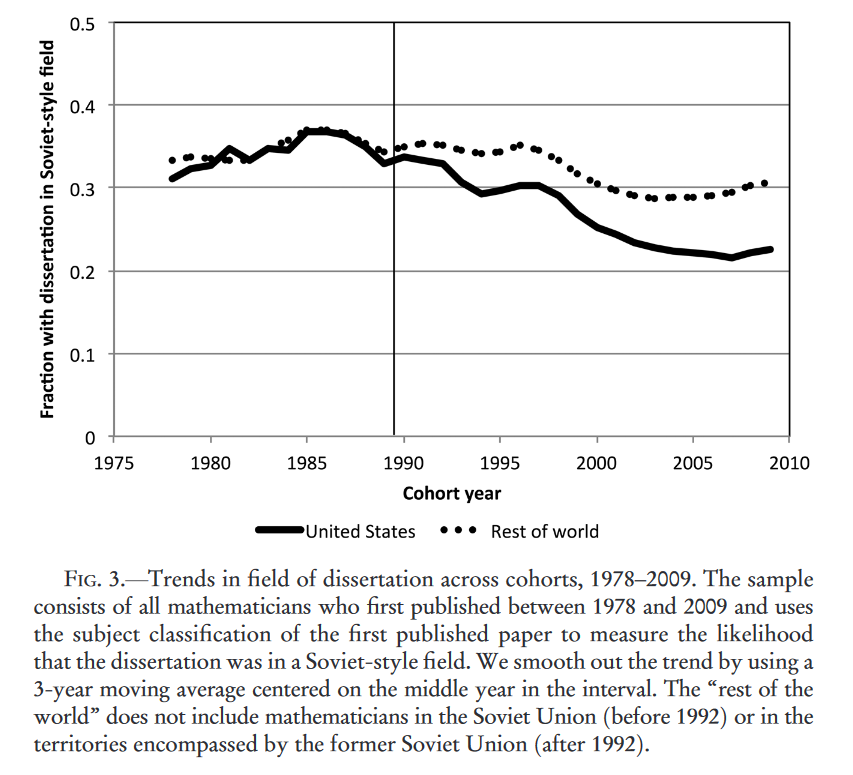
\includegraphics[width = \linewidth]{_images/0918sugiyama/Figure_3.png}
        \caption{Figure 3. Trends in field of dissertation across cohort}
        \label{fig:my_label}
    \end{figure}
    
    Table 8 illustrate the results of regression estimation.
    \begin{figure}
        \centering
        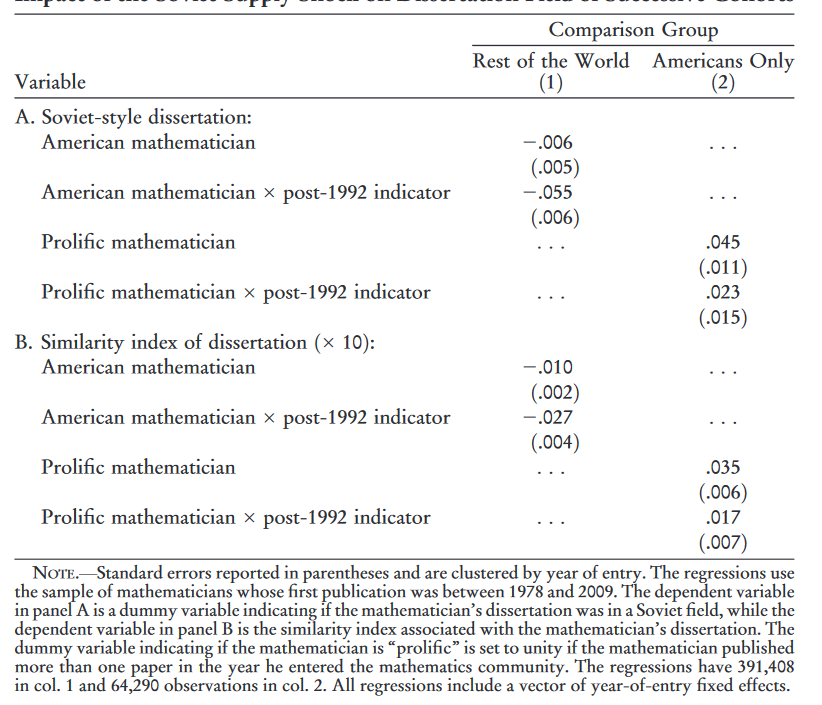
\includegraphics[width = \linewidth]{_images/0918sugiyama/Table_8.png}
        \caption{Figure 3. Trends in field of dissertation across cohort}
        \label{fig:my_label}
    \end{figure}
    
    \begin{itemize}
        \item The dependent variable is an index Soviet-ness of particular a dissertation.
        \item The results both column 1 and 2 show the number of mathematicians who wrote Soviet-style dissertation paper was decreased after 1992.
    \end{itemize}
    .
    Figure 4 illustrate the fraction of the mathematicians who publish at least one Soviet-style paper during specific year. 
    \begin{figure}
        \centering
        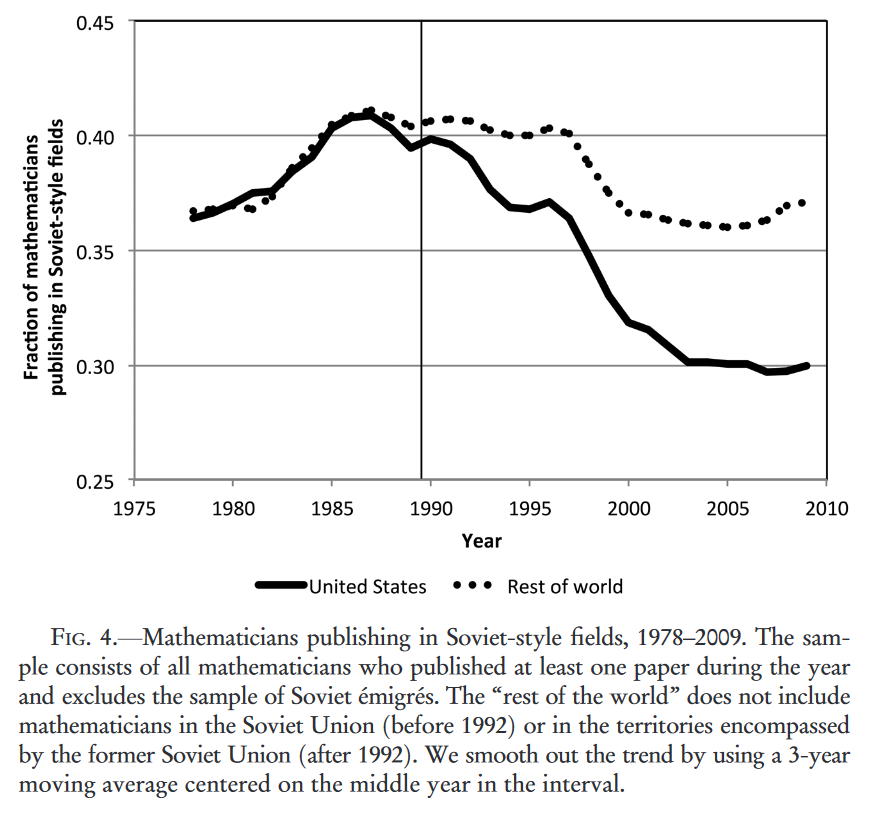
\includegraphics[width = \linewidth]{_images/0918sugiyama/Figure_4.png}
        \caption{Figure 4. Mathematicians published Soviet-style paper, 1978-2009}
        \label{fig:my_label}
    \end{figure}
    
    Figure 4 show the number of mathematicians also decreased after 1992.
    \section{Summary}
    
    \begin{itemize}
        \item Soviet supply shock made American math field competition more harder.  
        \item High-ability American mathematicians did not move to other field. This result suggest high-ability mathematicians benefit by inflow spillover. 
        \item Newcomers avoided to choose Soviet-style topic.
    \end{itemize}
    The authors focus on the knowledge production function in a very    specific marketplace: academia.
    
    They suspect that further study of the process cognitive mobility will lead to a greater understanding of knowledge spillover.  
    \biblio
    
\end{document}